\subsection{Respuesta al impulso}
Cuando $v_i(t) = \delta(t), V_i(s) = 1$. Por lo tanto, basta con calcular la transformada inversa de Laplace de $V_o(s) = H(s)$. Para ello se procede a realizar fracciones simples de $V_o(s)$
$$
V_o(s) = \frac{A}{s-p_1} + \frac{B}{s-p_2} + \frac{C}{s-p_3} + \frac{D}{s-p_4}
$$
\vskip0.5cm
Donde:
$$
A = Res(V_o(s), p_1) = \frac{0.8911 p_1^4}{(p_1-p_2)(p_1-p_3)(p_1-p_4)} = -1105 + 439j
$$
$$
B = Res(V_o(s), p_2) = \frac{0.8911 p_2^4}{(p_2-p_1)(p_2-p_3)(p_2-p_4)} = -1105 - 439j
$$
$$
C = Res(V_o(s), p_3) = \frac{0.8911 p_3^4}{(p_3-p_1)(p_3-p_2)(p_3-p_4)} = -26 - 137j
$$
$$
D = Res(V_o(s), p_4) = \frac{0.8911 p_4^4}{(p_4-p_1)(p_4-p_2)(p_4-p_3)} = -26 + 137j
$$
\vskip0.5cm
Por otro lado, tenemos que $\mathcal{L}^{-1}(\frac{1}{s-a}) = e^{at}$, por lo que resulta que:
$$
v_o(t) = A \cdot e^{p_1t} + B \cdot e^{p_2t} + C \cdot e^{p_3t} + D \cdot D e^{p_4t}
$$
\vskip0.5cm
Y como $ A = \overline{B}$, $C = \overline{D}$ y además $p_1 = \overline{p_2}$, $p_3 = \overline{p_4}$, entonces se tiene que:
$$
v_o(t) = 2\Re(A \cdot e^{p_1t}) + 2\Re(C \cdot e^{p_3 t})
$$
\vskip0.5cm
Por lo tanto se obtiene:
\begin{align*}
    v_o(t) & = -2210.14 cos(1374.31t)e^{-1136.16t} -878.06sen(1374.31t)e^{-1136.16t}\\
           & + -52 cos(939.5t) e^{-133.34t} + 274 sen(939.5t)e^{-133.34t}
\end{align*}

\begin{figure}[H]
    \centering
    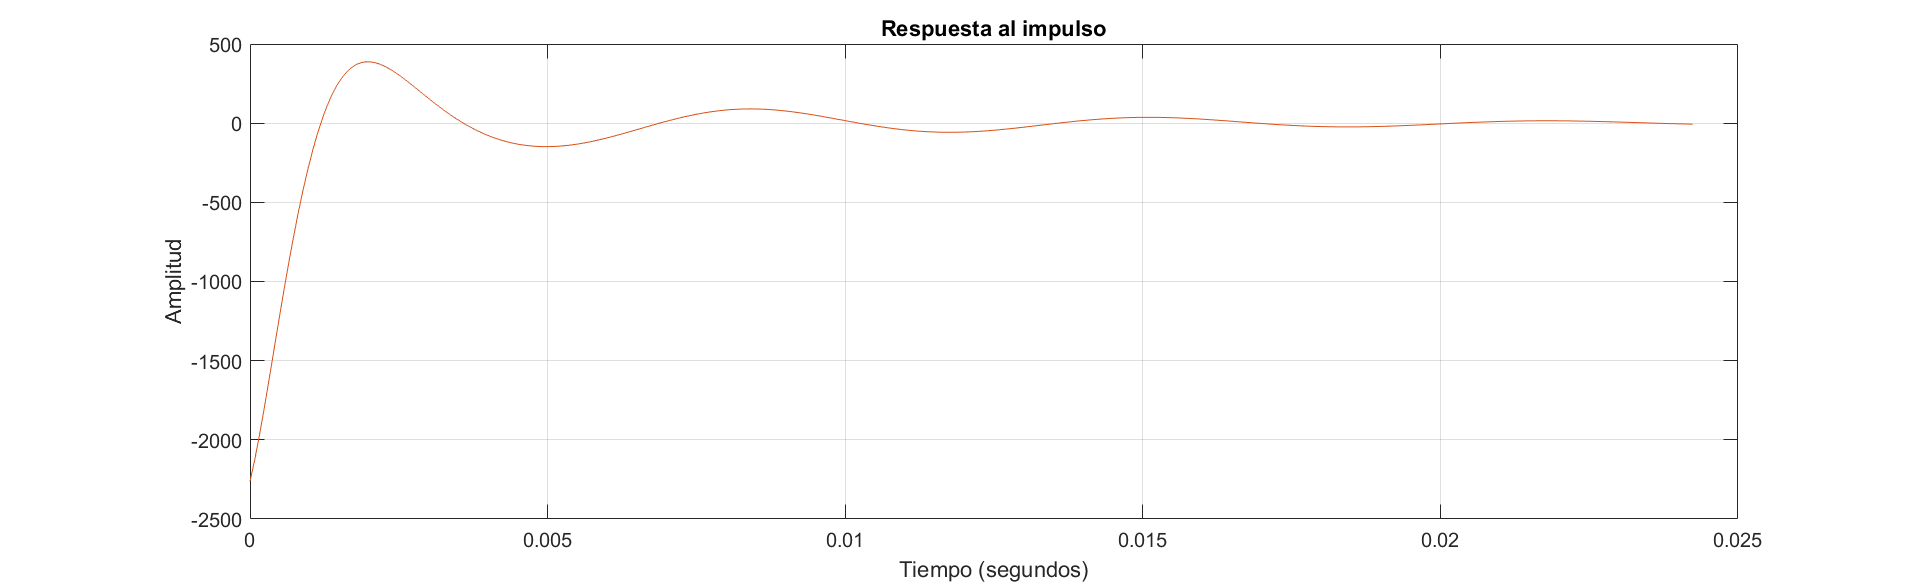
\includegraphics[width=1\textwidth]{resources/RespuestaAlImpulso.png}
    \caption{Respuesta al impulso}
\end{figure} 

\subsection{Respuesta al escalón}
Cuando $v_i(t) = \Delta(t)$, siendo $\Delta(t)$ la función escalón de Heaviside, entonces se tiene que $V_i(s) = \frac{1}{s}$. Por lo tanto, basta con calcular la transformada inversa de Laplace de
$$
V_o(s) = \frac{1}{s} H(s) = \frac{0.8911 s^3}{s^4 + 2539 s^3 + 4.686 \cdot 10^6 s^2 + 2.894 \cdot 10^9 s + 2.863 \cdot 10^{12}}$$
\vskip0.5cm
Para ello se procede a realizar fracciones simples de $V_o(s)$

$$
V_o(s) = \frac{A}{s-p_1} + \frac{B}{s-p_2} + \frac{C}{s-p_3} + \frac{D}{s-p_4}
$$
\vskip0.5cm
Donde:
$$
A = Res(V_o(s), p_1) = \frac{0.8911 p_1^3}{(p_1-p_2)(p_1-p_3)(p_1-p_4)} = 0.5846 + 0.3208j
$$
$$
B = Res(V_o(s), p_2) = \frac{0.8911 p_2^3}{(p_2-p_1)(p_2-p_3)(p_2-p_4)} = 0.5846 - 0.3208j
$$
$$
C = Res(V_o(s), p_3) = \frac{0.8911 p_3^3}{(p_3-p_1)(p_3-p_2)(p_3-p_4)} = -0.1391 + 0.0476j
$$
$$
D = Res(V_o(s), p_4) = \frac{0.8911 p_4^3}{(p_4-p_1)(p_4-p_2)(p_4-p_3)} = -0.1391 - 0.0476j
$$
\vskip0.5cm
Por lo tanto,

\begin{align*}
    v_o(t) & = 1.1692cos(1374.31t)e^{-1136.16t} - 0.6416sen(1374.31t)e^{-1136.16t}\\
           & + -0.2782cos(939.5t)e^{-133.34t} -0.094sen(939.5t)e^{-133.34t}
\end{align*}

\begin{figure}[H]
    \centering
    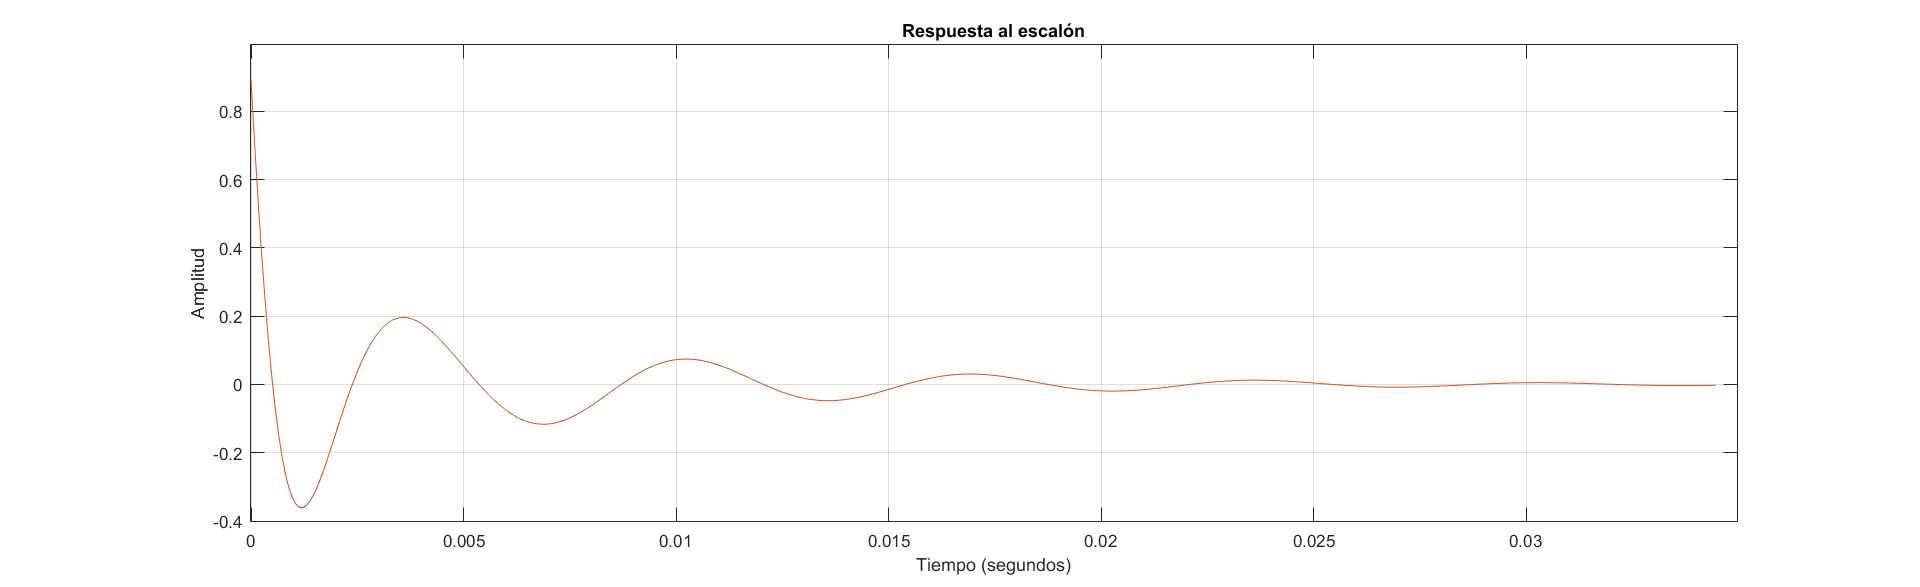
\includegraphics[width=1\textwidth]{resources/RespuestaAlEscalon.png}
    \caption{Respuesta al escalón}
\end{figure}


\subsection{Respuesta a la señal sinusoidal (frecuencia de corte)}
Dado que $\mathcal{L}(sen(\omega t)) = \frac{\omega}{\omega^2+s^2}$, y tomando $\omega = \omega_0 = 895.3 \frac{rad}{s}$. Para obtener la salida del filtro será necesario realizar la transformada inversa de Laplace de

$$
    V_o = \frac{895.3}{895.3^2+s^2} \cdot H(s) = \frac{797.8 s^4}{(s^4 + 2539 s^3 + 4.686 \cdot 10^6 s^2 + 2.894 \cdot 10^9 s + 2.863 \cdot 10^{12})(s^2+895.3^2)}
$$

Ahora, los polos serán:
$$
    p_1 = -1136.16 + 1374.31j
$$
$$
    p_2 = -1136.16 - 1374.31j
$$
$$
    p_3 = -133.34 + 939.50j
$$
$$
    p_4 = -133.34 - 939.50j
$$
$$
    p_5 = 895.3j
$$
$$
    p_6 = -895.3j
$$
\vskip0.5cm
Por lo tanto:
\vskip0.5cm
$$
V_o(s) = \frac{A}{s-p_1} + \frac{B}{s-p_2} + \frac{C}{s-p_3} + \frac{D}{s-p_4} + \frac{E}{s-p_5} + \frac{F}{s-p_6}
$$
\vskip0.5cm
Siendo los coeficientes:
\vskip0.5cm
$$
A = Res(V_o(s), p_1) = \frac{797.8 p_1^4}{(p_1-p_2)(p_1-p_3)(p_1-p_4)(p_1-p_5)(p_1-p_6)} = -0.1459 - 0.3073j
$$
$$
B = Res(V_o(s), p_2) = \frac{797.8 p_2^4}{(p_2-p_1)(p_2-p_3)(p_2-p_4)(p_2-p_5)(p_2-p_6)} = -0.1459 + 0.3073j
$$
$$
C = Res(V_o(s), p_3) = \frac{797.8 p_3^4}{(p_3-p_1)(p_3-p_2)(p_3-p_4)(p_3-p_5)(p_3-p_6)} = 0.4825 + 0.0284j
$$
$$
D = Res(V_o(s), p_4) = \frac{797.8 p_4^4}{(p_4-p_1)(p_4-p_2)(p_4-p_3)(p_4-p_5)(p_4-p_6)} = 0.4825 - 0.0284j
$$
$$
E = Res(V_o(s), p_5) = \frac{797.8 p_5^4}{(p_5-p_1)(p_5-p_2)(p_5-p_3)(p_5-p_4)(p_5-p_6)} = -0.3365 + 0.1097j
$$
$$
F = Res(V_o(s), p_6) = \frac{797.8 p_6^4}{(p_6-p_1)(p_6-p_2)(p_6-p_3)(p_6-p_4)(p_6-p_5)} = -0.3365 - 0.1097j
$$
\vskip0.5cm
Y nuevamente por propiedades de números complejos conjugados:
\vskip0.5cm
$$
    v_o(t) = 2\Re(Ae^{p_1t}) + 2\Re(Ce^{p_3t}) + 2\Re(Ee^{p_5t})
$$
\vskip0.5cm

\begin{align*}
    v_o(t) & = e^{-1136.16t} \cdot (-0.2918 \cdot cos(1374.31t) + 0.6146 \cdot sen(1374.31t)) \\
           & + e^{-133.34t} \cdot (0.965 \cdot cos(939.5t) - 0.0568 \cdot sen(939.5t)) \\
           & - 0.673 \cdot cos(895.3t) - 0.2194 \cdot sen(895.3t)
\end{align*}

\begin{figure}[H]
    \centering
    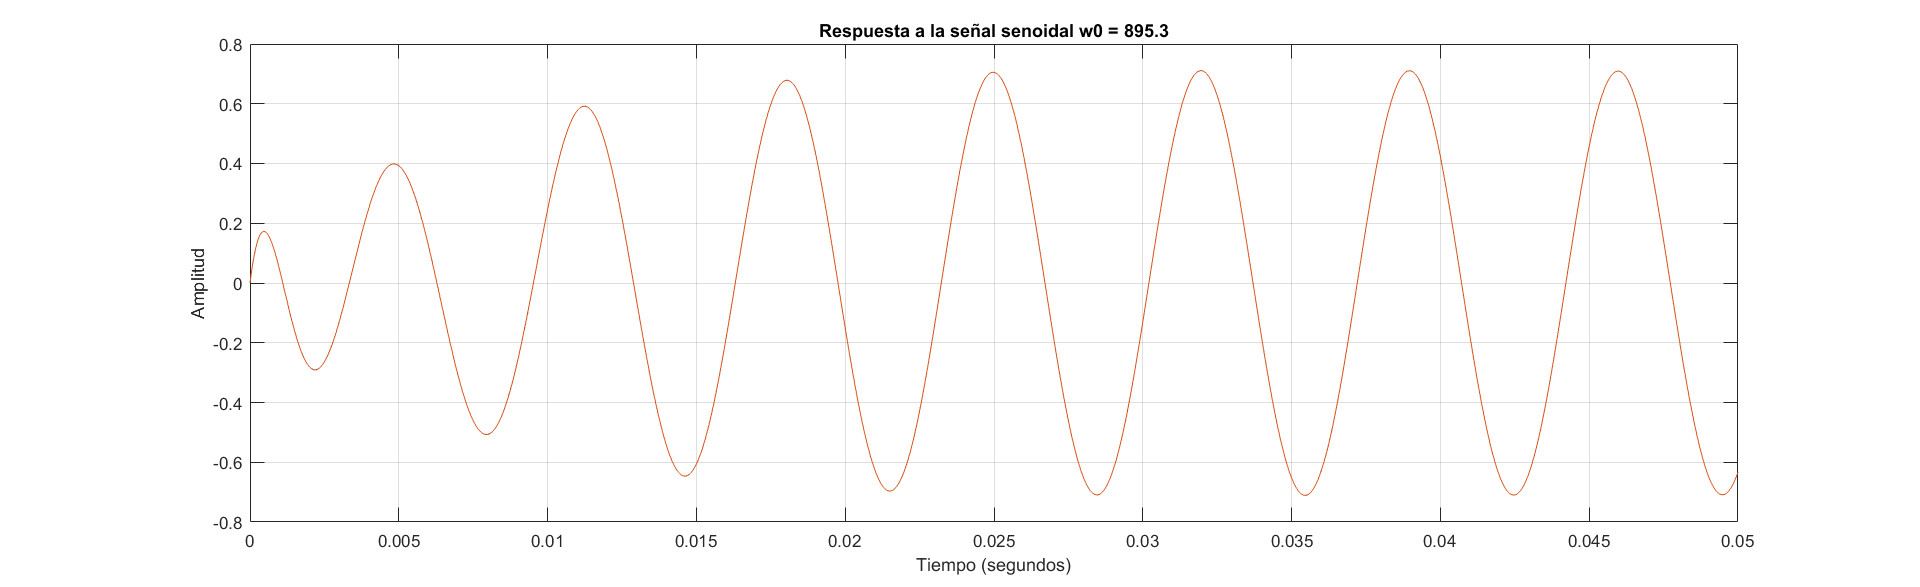
\includegraphics[width=1\textwidth]{resources/RespuestaAlSinusoide.png}
    \caption{Respuesta a la señal senoidal}
\end{figure}